\subsection{Comparing different lifting operators}\label{sec:mesh_motion}
This section is devoted to comparing different lifting operators from \ref{sec:meshmotion}. The comparisions will be run using a version of the CSM test discussed earlier, with the same computing domain as the Hron Turek benchmark. The tests will compare the different techniques by looking at the how the deformation is lifted into the fluid domain. This is done by investigating a plot of the mesh after deformation to see how much cells distort and where the cells distort. This is visualized using Paraview.\newline
In these test cases we have the fluid initially at rest and with no inflow on the fluid. A gravitational force is applied to the structure much like the previous CSM test. The only difference is that we now use the full domain from the \ref{sec:HronTurek} . The tests are run as time-dependent with a the backward Euler scheme, leading to a steady state solution. In the first test case the parameters from CSM1 are used, and in the CSM4 the gravitational force has just been increased from 2 to 4. \newline

A plot has been added at the end of the FSI2 case run with different techniques to investigate the impact these have on the overall FSI problem.

\subsection*{Boundary conditions}
The upper, lower and left boundary is set as no slip, that is no velocity in the fluid. On the left boundary there is a do nothing, and zero pressure. 
\subsection*{Quantities for comparison}
The different techniques will be plotted with the minimal value of the Jacobian. The Jacobian determinant of the deformation rate, and \textbf{if the Jacobian is zero anywhere in the domain it means that the cells overlap and can cause singularity in the matrices during assembly.} \newline
We will also look at the a plot of the deformation in the domain, to visualize how the different mesh motion techniques work. It is possible to see that if get thin triangles in the computational domain then the lifting operator is not good enough.
\subsubsection*{Different lifting operators with testcase CSM1}
\begin{figure}[H]
\label{fig:fluid_structure}
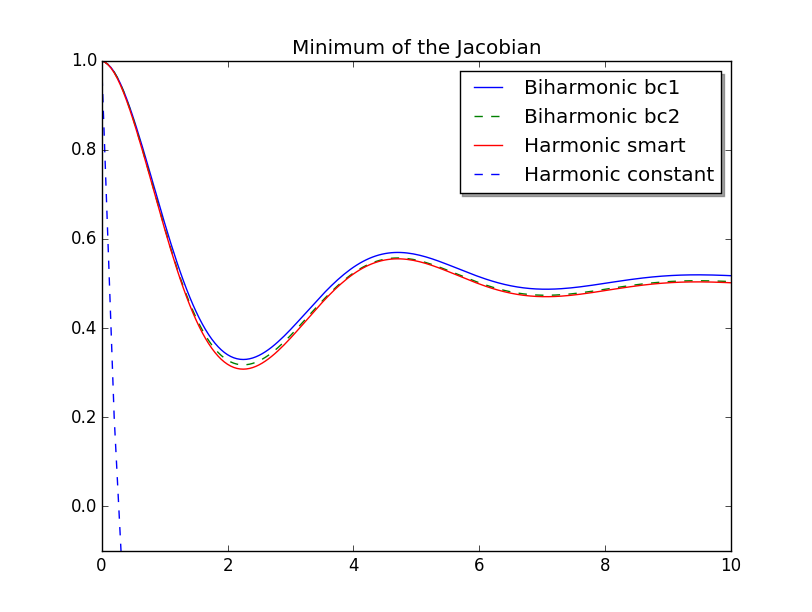
\includegraphics[scale=0.60, trim={0mm 0mm 0mm 0mm},clip]{./Verification_Validation/Mesh_motion_results/CSM1.png}
\caption{plot of the minimum of J in entire domain, using CSM1 test. $\Delta t = 0.05$}
\end{figure}

\begin{figure}[H]  \label{fig:CSM1_pictures} 
  \caption{Results of testing different lifting operator using the CSM1 testcase computing full FSI}
  \begin{minipage}[b]{0.6\linewidth}
    \centering
    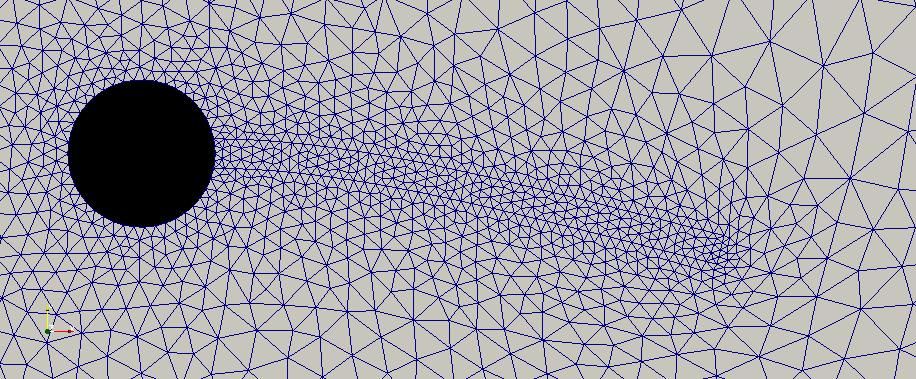
\includegraphics[scale=0.25]{./Verification_Validation/Mesh_motion_results/CSM1_laplace.png} 
    \caption{Harmonic smart} 
    \vspace{4ex}
  \end{minipage}%%
  \begin{minipage}[b]{0.6\linewidth}
    \centering
    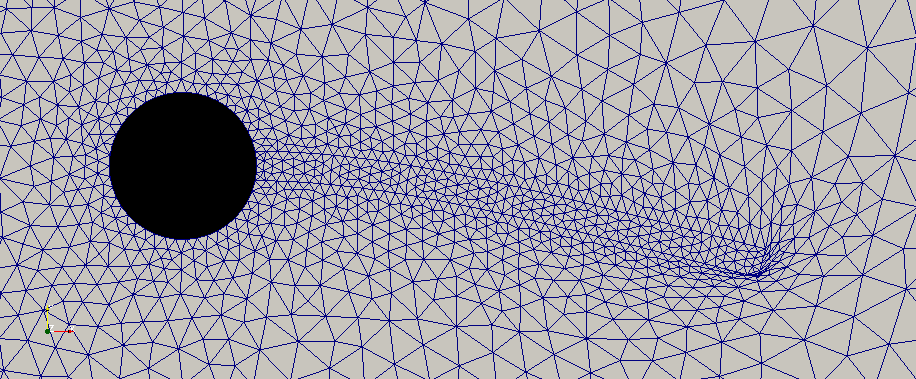
\includegraphics[scale=0.25]{./Verification_Validation/Mesh_motion_results/CSM1_constant.png} 
    \caption{Harmonic constant} 
    \vspace{4ex}
  \end{minipage} 
  \begin{minipage}[b]{0.6\linewidth}
    \centering
    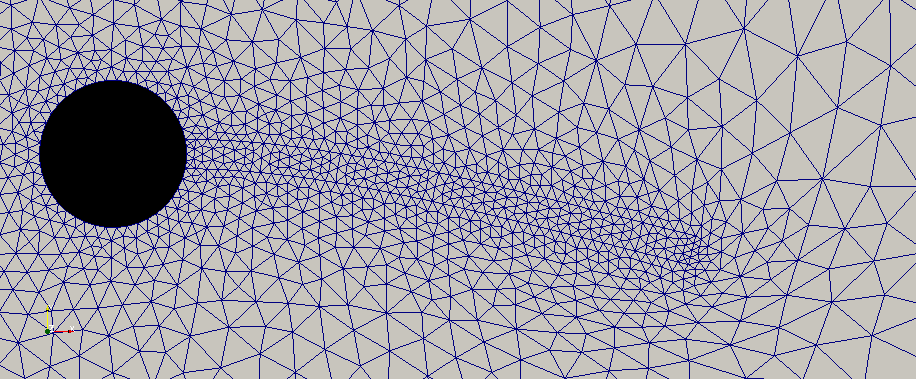
\includegraphics[scale=0.25]{./Verification_Validation/Mesh_motion_results/CSM1_bibc1.png} 
    \caption{Biharmonic bc1} 
    \vspace{4ex}
  \end{minipage}%% 
  \begin{minipage}[b]{0.6\linewidth}
    \centering
    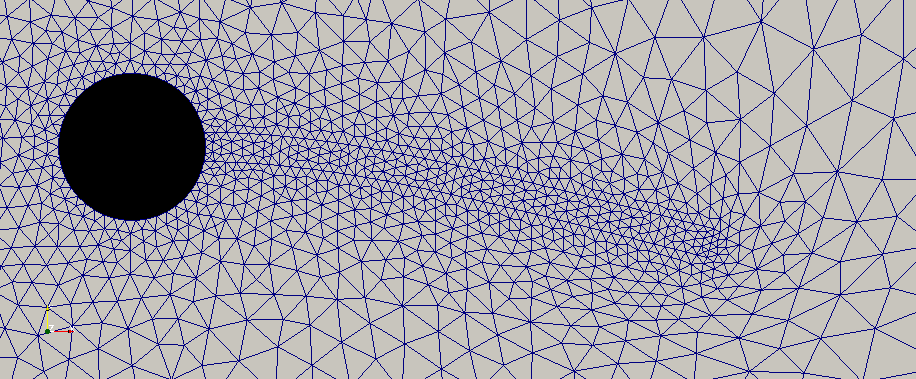
\includegraphics[scale=0.25]{./Verification_Validation/Mesh_motion_results/CSM1_bibc2.png} 
    \caption{Biharmonic bc2} 
    \vspace{4ex}
  \end{minipage} 
\end{figure}



\begin{table}[H]
\centering
\caption{Displacements results of different lifting operators of CSM1 test}
\label{my-label}
\begin{tabular}{|l|l|l|}
\hline
Technique & $d_y(A) [\times 10^{-3}]$ & $d_x(A) [\times 10^{-3}]$ \\ \hline
Harmonic & 65.406 & 7.036 \\ \hline
Constant & 43.033 & 2.999 \\ \hline
Bibc1 & 65.404 & 7.036 \\ \hline
Bibc2 & 65.405 & 7.036 \\ \hline
\end{tabular}
\end{table}


Looking at figure \ref{fig:fluid_structure} which shows the minimum of the Jacobian of the entire domain. The Harmonic with a constant $\alpha_u$ parameter. Gives overlapping cells quickly and computations stop.
While the harmonic named smart meaning an $\alpha_u$ that is greater closer to the interface, and both the biharmonic techniques gives good and similar results. All three uphold, as we can see in \ref{fig:CSM1_pictures}, the integrity of the cells.


\subsubsection{FSI2 with Lifting operator}

\begin{figure}[H]  \label{fig:FSI2_motion} 
  \begin{minipage}[b]{0.6\linewidth}
    \centering
    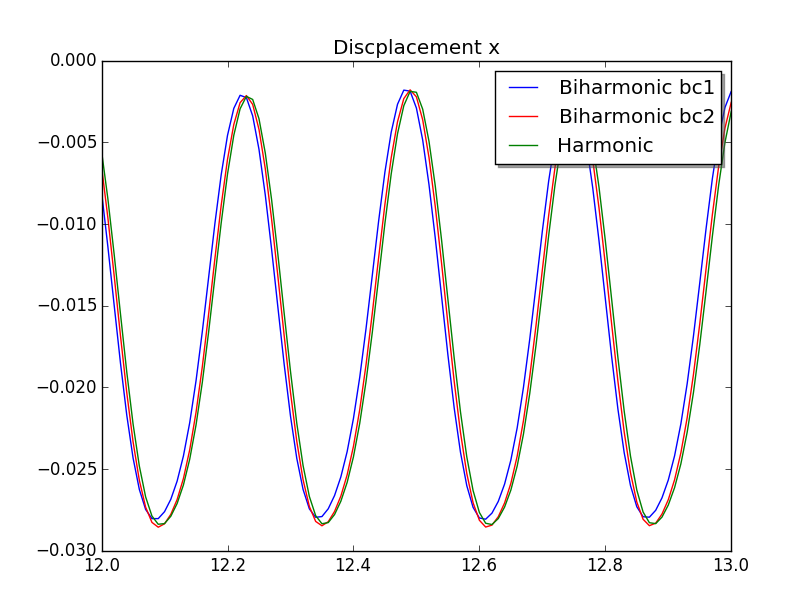
\includegraphics[scale=0.41]{./Verification_Validation/Mesh_motion_results/FSI2_dt001_dis_x.png} 
    \vspace{4ex}
  \end{minipage}%%
  \begin{minipage}[b]{0.6\linewidth}
    \centering
    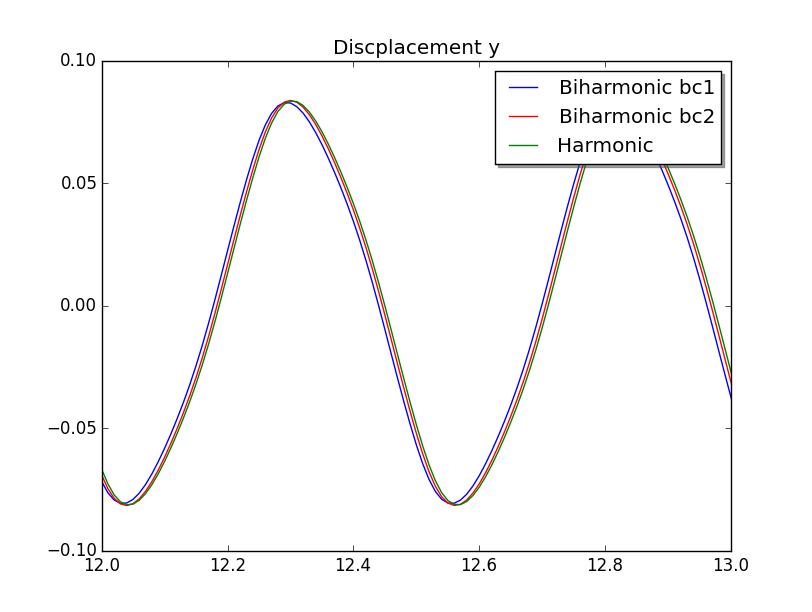
\includegraphics[scale=0.41]{./Verification_Validation/Mesh_motion_results/FSI2_dt001_dis_y.png} 
    \vspace{4ex}
  \end{minipage} 
  \begin{minipage}[b]{0.6\linewidth}
    \centering
    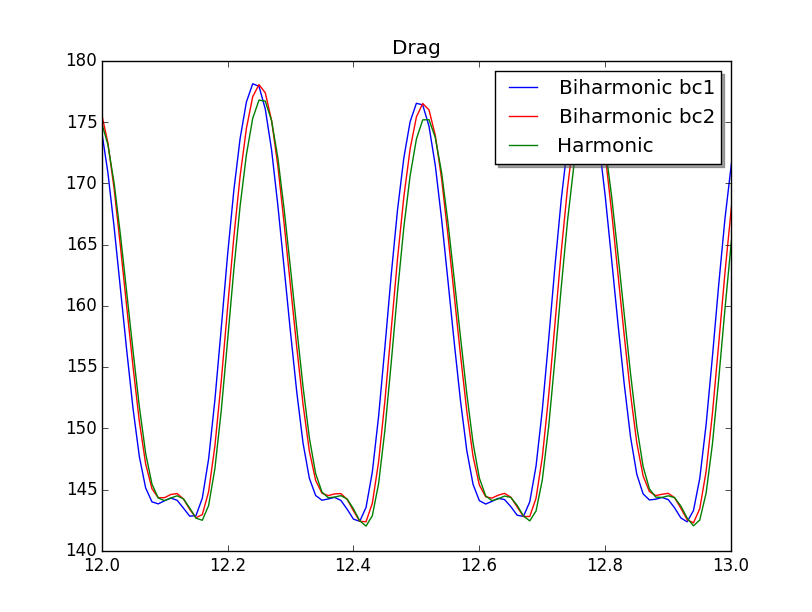
\includegraphics[scale=0.41]{./Verification_Validation/Mesh_motion_results/FSI2_dt001_drag.png} 
    \vspace{4ex}
  \end{minipage}%% 
  \begin{minipage}[b]{0.6\linewidth}
    \centering
    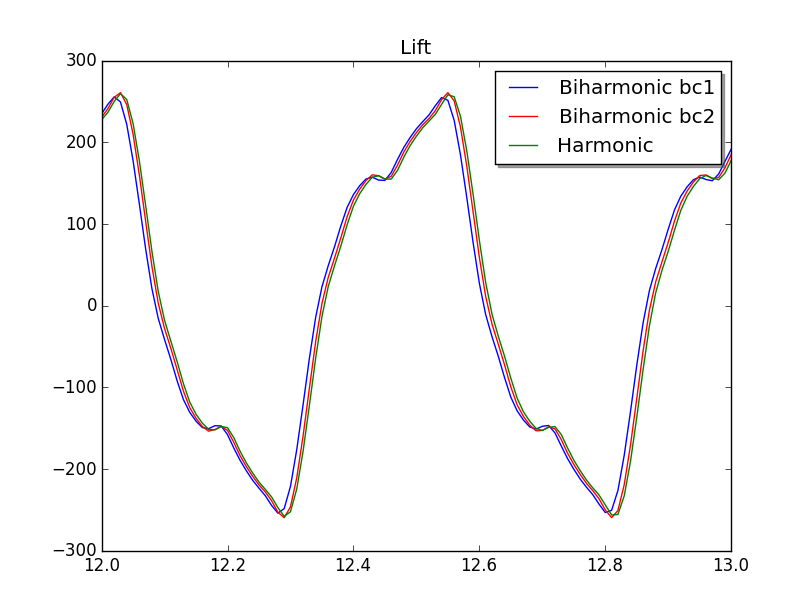
\includegraphics[scale=0.41]{./Verification_Validation/Mesh_motion_results/FSI2_dt001_lift.png} 
    \vspace{4ex}
  \end{minipage} 
\caption {FSI2 with different lifting operators: Harmonic, Biharmonic bc1 and bc2. $\Delta t = 0.01$}
\end{figure}

Figure \ref{fig:FSI2_motion} shows the harmonic and the two biharmonic mesh motion techniques for the FSI2 case. All three are similar and only a slight change in the period can be noticed. This indicates that with a clever $\alpha_u$ the harmonic technique can be chosen. This is an advantage since the harmonic techniques is the least computationally costly.








